% vim: set tw=78 sts=2 sw=2 ts=8 aw et ai:
\documentclass[12pt]{article}

\usepackage[paper=a4paper, top=2cm, bottom=3cm, left=2.5cm, right=2.5cm]{geometry}

\usepackage{ucs}
\usepackage[utf8x]{inputenc}
\usepackage[english]{babel}
\usepackage{underscore}	  % underscores need not be escaped
\usepackage{subfigure}
\usepackage{verbatim}
\usepackage{float}
\usepackage{booktabs}     % professional tables
\usepackage{parskip}      % paragraph spacing
\usepackage{setspace}     % line spacing

% Support for including graphics
\usepackage{graphicx}
\DeclareGraphicsExtensions{.pdf,.png,.jpg}

% Code listings support
\usepackage{listings}
\lstnewenvironment{file-content}[1][]%
  {\minipage{\linewidth} 
   \lstset{
	numbers=left, numberstyle=\footnotesize,
	frame=lines, captionpos=b,
	breaklines=true,
	basicstyle=\ttfamily,#1
   	}}
  {\endminipage}

\usepackage{hyperref}	  % use \url{http://$URL} or \href{http://$URL}{Name}
\hypersetup{%
	colorlinks=true,
	linkcolor=black,
	anchorcolor=black,
	citecolor=black,
	filecolor=black,
	menucolor=black,
	urlcolor=black,
	bookmarks=black,
	bookmarksnumbered=black
}
% commands for creating labeled hyper-linked references
\newcommand{\labelindexref}[2]{\hyperref[#2]{#1~\ref*{#2}}}
\newcommand{\labelref}[2]{\hyperref[#2]{#1}}

\title{Peer-To-Peer Virtual Private Networks:\\
Multiple Supernodes Feature for N2N}

\author{Costin Lupu\\
Automatic Control and Computers Faculty\\
University POLITEHNICA of Bucharest\\
Splaiul Independenței nr. 313, Bucharest, Romania \\
\emph{costin.lup@gmail.com}}

\date{\today}

\begin{document}

\maketitle

\begin{abstract}
% vim: set tw=78 sts=2 sw=2 ts=8 aw et ai:
The current research report describes the design and implementation of a decentralizing enhancement technique applied for N2N, a Peer-to-Peer Virtual Private Network solution. The feature addresses two important points for distributed systems: reliability and availability.

\end{abstract}

\section{Introduction}
\label{sec:introduction}
% vim: set tw=78 sts=2 sw=2 ts=8 aw et ai:
\onehalfspacing
N2N (network to network)\cite{n2n_paper} is a layer-two over layer-three P2P virtual private network (VPN) application which allows users to exploit properties typical of P2P applications at the network level instead of application level. This means that users can gain unrestricted IP visibility and be reachable with the same address regardless of their current network environment. In a nutshell, as OpenVPN moved SSL \cite{tls} from application (e.g. used to implement the https protocol) to network protocol, N2N moves P2P from application to network level.

Like most P2P protocols, N2N has one or more supernodes and several edge nodes. Supernodes are used to introduce edge nodes and to cross symmetric NAT. Edge-nodes are grouped in communities coordinated by the supernode. Periodically an edge-node sends registration messages to supernode for keeping its record in the supernode peers list. A backup supernode can be assigned to each edge as a command line parameter which will be used if the connection with main supernode fails.


\section{Multiple Supernodes - Overview}
\label{sec:overview}
% vim: set tw=78 sts=2 sw=2 ts=8 aw et ai:

The current N2N versions uses a very limited set of supernodes that are provided on edges startups as command line parameters. Furthermore, there is no communication between supernodes for distributing the lists of communities and/or edges. As a result, in order to communicate with each other, 2 edges in the same community must register to the same supernode. This also implies that for the current version of N2N the supernode becomes a single point of failure, making the whole virtualized network vulnerable. If the supernodes that were used on edge registration stop running, the whole network setup is lost.

Due to its performances and size, N2N can be also used on mesh mobile or wireless sensor networks. However, different mesh networks cannot be interconnected as long as their coordinating nodes, the supernodes in the N2N case, don't have a communication protocol. For a set of low power mobile nodes it is essential that the communication with the coordinating node to be established based on connectivity performance.

Another key factor for improving communication, especially when relaying is necessary, is load-balancing: the communities should be equally distributed among the set of supernodes based on their edges number and response times.

The problems outlined above raised the demand on the N2N discussion list \cite{demand} for implementing multiple supernodes functionality for N2N. The N2N creators suggested the following basic functions would be needed in edge \cite{suggestions}:
\begin{itemize}
\item Detecting that a supernode has failed
\item Avoiding use of failed supernodes
\item Detecting supernode recovery
\item Reinstating use of a recovered supernode
\end{itemize}
Also, regarding feature design, the authors outlined two major concerns: supernode discovery and packet forwarding behaviour. The options suggested for the former were either all edges in a community are statically configured to use the same set of supernodes, or supernodes can be discovered from any one supernode in the group. The options for packet forwarding behaviour were:
\begin{itemize}
\item All edges in a community must stay connected to the complete set of supernodes so that any supernode is able to forward packets between any two edges.
\item Edges can have different supernode connectivity and the supernodes manage forwarding packets to a supernode that has an open connection to the destination edge.
\end{itemize}
The current feature implementation includes dynamic supernode discovery. However, for packet forwarding, the chosen solution was keeping all edges in community connected to the subset of coordinating supernodes. The feature design had to be determined from two perspectives: inter-community and intra-community.

Inter-community perspective involved designing the communication between supernodes under a new protocol, on a different port than the one used for the N2N communication protocol. This approach was chosen because the messages of the N2N protocol are edge oriented, each message header containing the community name of the initiating node. The main goal of supernode communication is distributing the peers communities. A starting supernode would have to choose some communities it would voluntarily coordinate, a decision being made depending on the needed level of redundancy for any given community. This stage will be further referred as communities discovery. Every supernode is represented by 2 pairs of addresses: \emph{IP address, UDP Port}. First one, used in the N2N protocol will be further referred as N2N address or advertise address, is the address on which a supernode is receiving edge registrations or performing relayed transfers for peers between symmetric NAT. Second one, used in the Multiple Supernodes protocol will be referred as SNM address.

Intra-community perspective implied choosing the messages to be exchanged between an edge-node and a supernode, before the former is ready to communicate with its peers. The main goal is establishing the set of supernodes that will be coordinating the community based on connection quality and supernodes load level. This stage will be further referred as supernodes discovery.

The feature was implemented \cite{git_repo} in order to alter as less as possible the current version of N2N and to allow further modifications to be made easily. Decisions regarding the design of the two types of communication will be argued next. In following sections of the report, the implemented protocol will be referred as Multiple Supernodes (SNM) protocol. 


\section{Message Formats}
\label{sec:message-formats}
% vim: set tw=78 sts=2 sw=2 ts=8 aw et ai:

\subsection{SNM Message Header}
\label{sub-sec:snm-header}
\labelindexref{Fig.}{img:snm-hdr} shows the header used in all SNM messages. \emph{Type} field holds an 1-byte value representing the message type. Current message types values are:
\begin{itemize}
\item \emph{0x01} – for SNM requests
\item \emph{0x02} – for SNM responses
\item \emph{0x03} – for SNM advertise messages
\end{itemize}
A message holding any other message type will be ignored. \emph{Flags} is a 1-byte value representing the flags associated with each message type. On every request, a 2-bytes \emph{Sequence Number} is generated by the issuer for keeping track of all sent messages.

\begin{figure}[hbtp]
\begin{center}
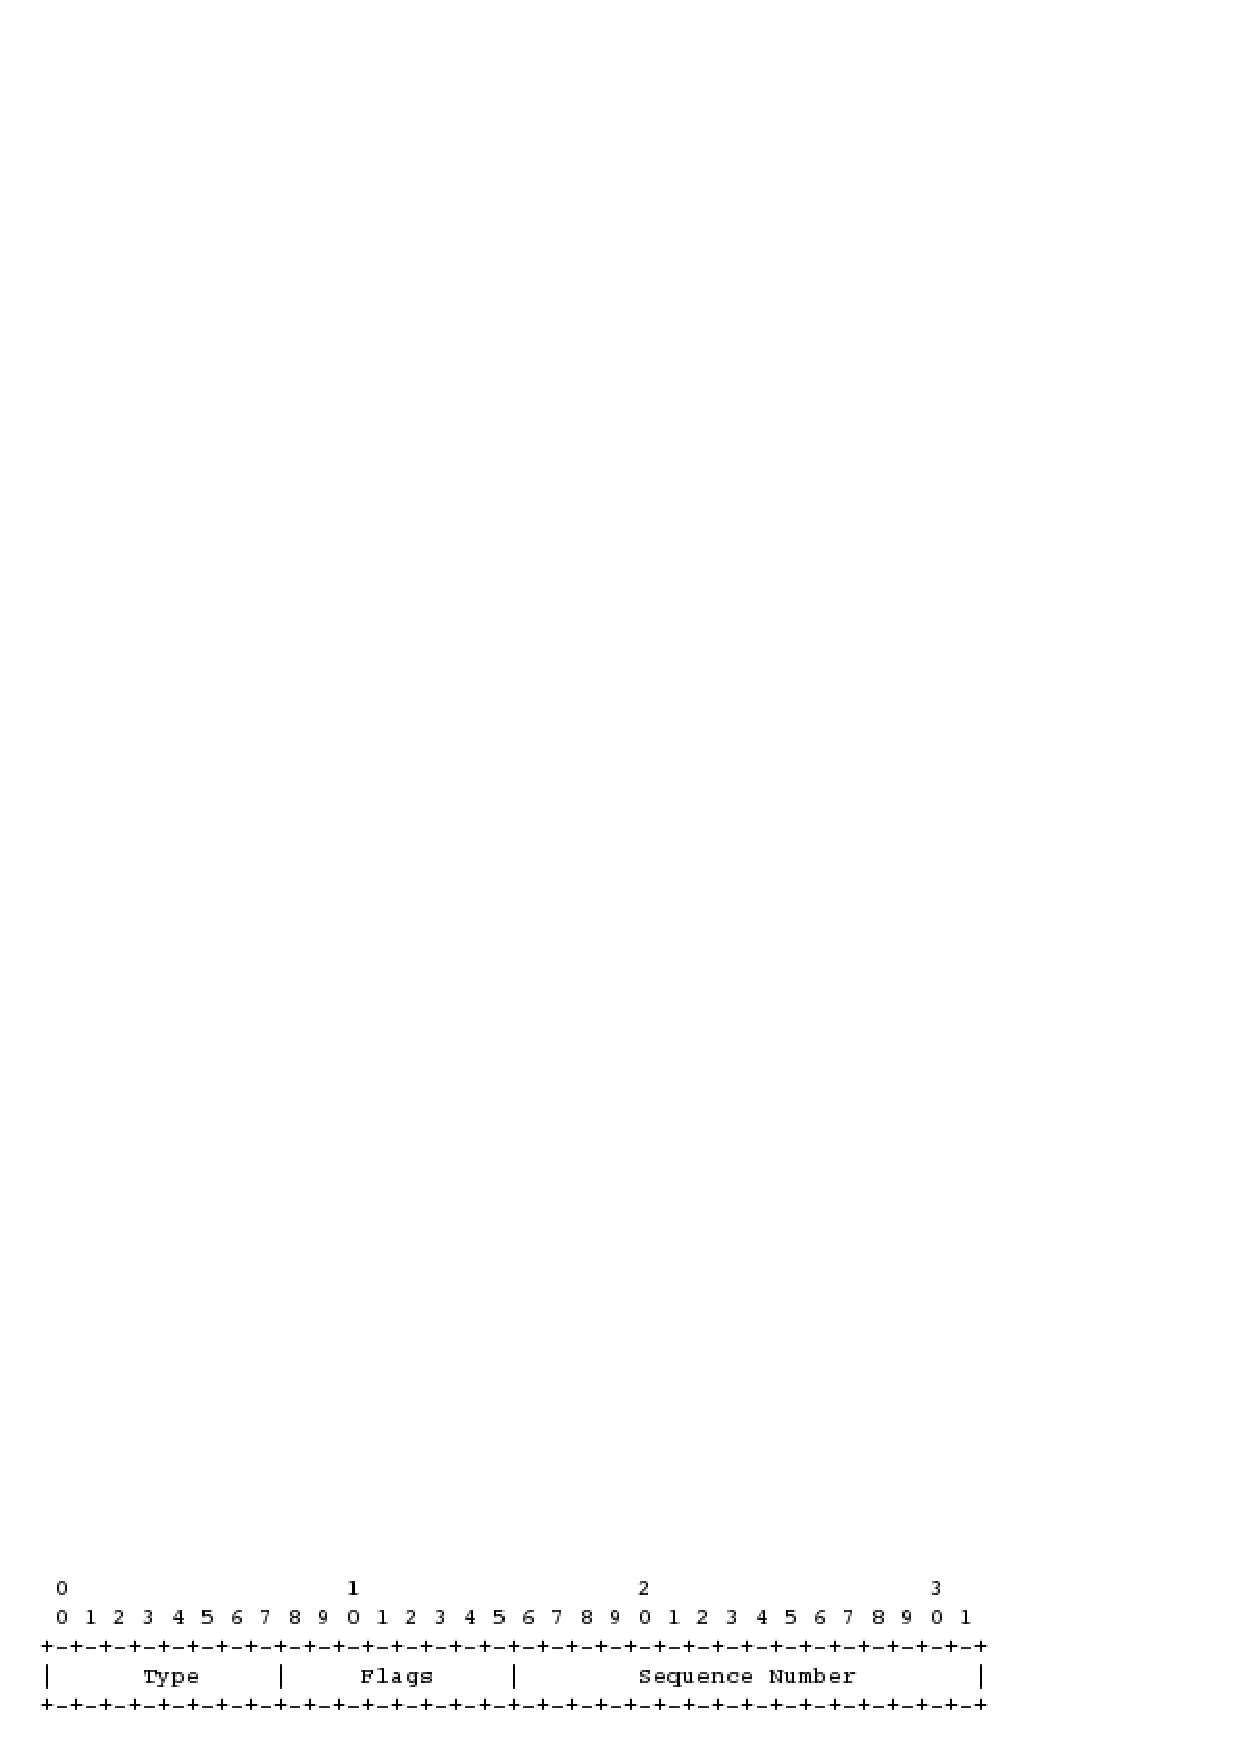
\includegraphics[scale=0.7]{img/snm-hdr.pdf}
\caption{SNM Message Header \label{img:snm-hdr}}
\end{center}
\end{figure}

\subsection{SNM Request Message}
\label{sub-sec:snm-request}
The request message flags have the following meanings:
\begin{itemize}
\item \emph{S} – all known SNM addresses of running supernodes are requested.
\item \emph{C} – all communities coordinated by the receiving supernode are requested.
\item \emph{N} – only SNM addresses of supernodes coordinating the provided communities are requested. The request payload will contain a list of community names. Every community name is filled as a variable-length name (name length followed by the string itself). \emph{N} and \emph{C} flags are mutually exclusive.
\item \emph{A} – the advertise address (N2N supernode address) is requested.
\item \emph{E} – message is initiated by an edge-node.
\end{itemize}

\begin{figure}[hbtp]
\begin{center}
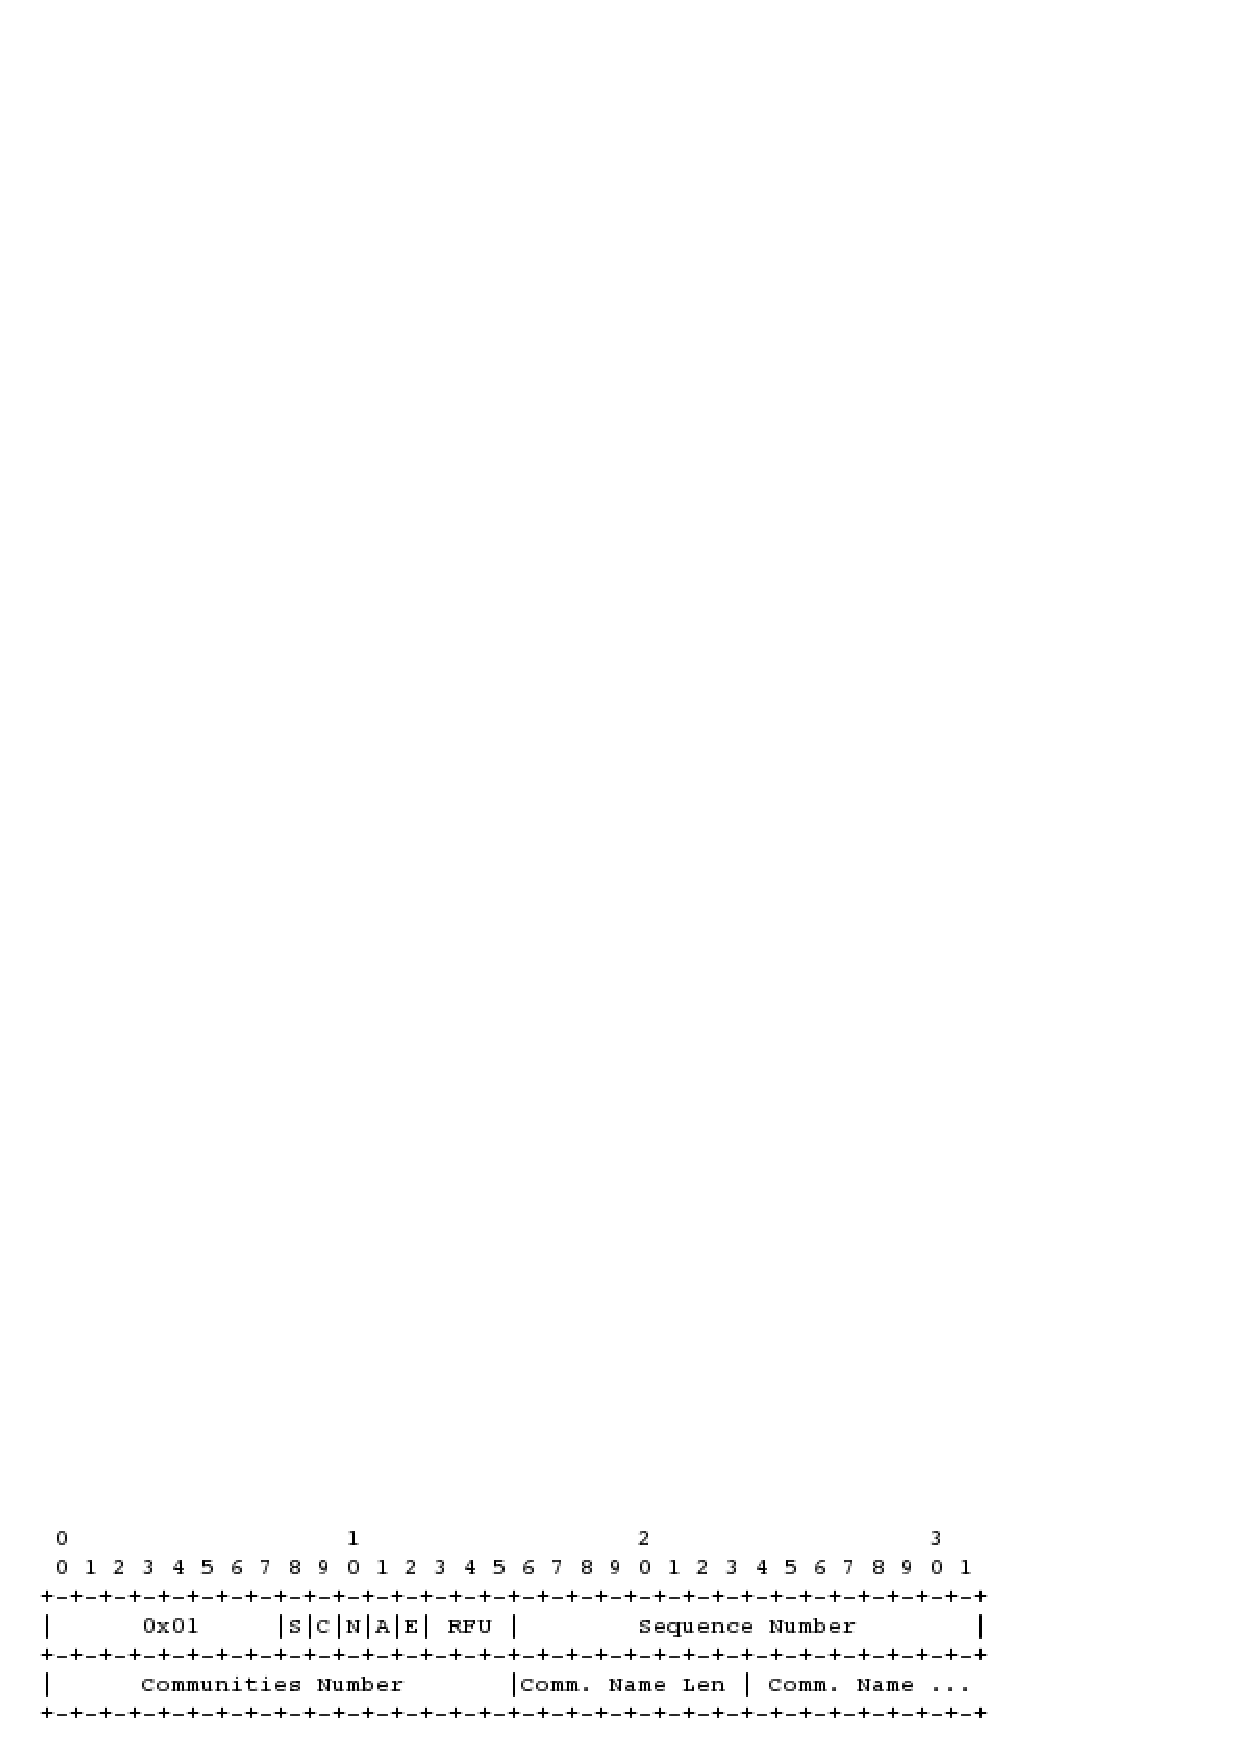
\includegraphics[scale=0.7]{img/snm-req.pdf}
\caption{SNM Request Message \label{img:snm-req}}
\end{center}
\end{figure}

\subsection{SNM Response Message}
\label{sub-sec:snm-response}
\labelindexref{Fig.}{img:snm-rsp} represents the message format of the SNM response message. A SNM response is always sent by a supernode in reply to a SNM request. \emph{Supernodes Number} and \emph{Communities Number} fields will be always set, regardless the type of request that was previously sent.
The supernodes addresses are encoded with the following fields:
\begin{itemize}
\item \emph{Family} – 1-byte value representing the IP protocol family (IPv4 or IPv6)
\item \emph{UDP Port} – 2-bytes value 
\item \emph{IP Address} – 4-bytes IPv4 address or 16-bytes IPv6 address 
\end{itemize}

\begin{figure}[hbtp]
\begin{center}
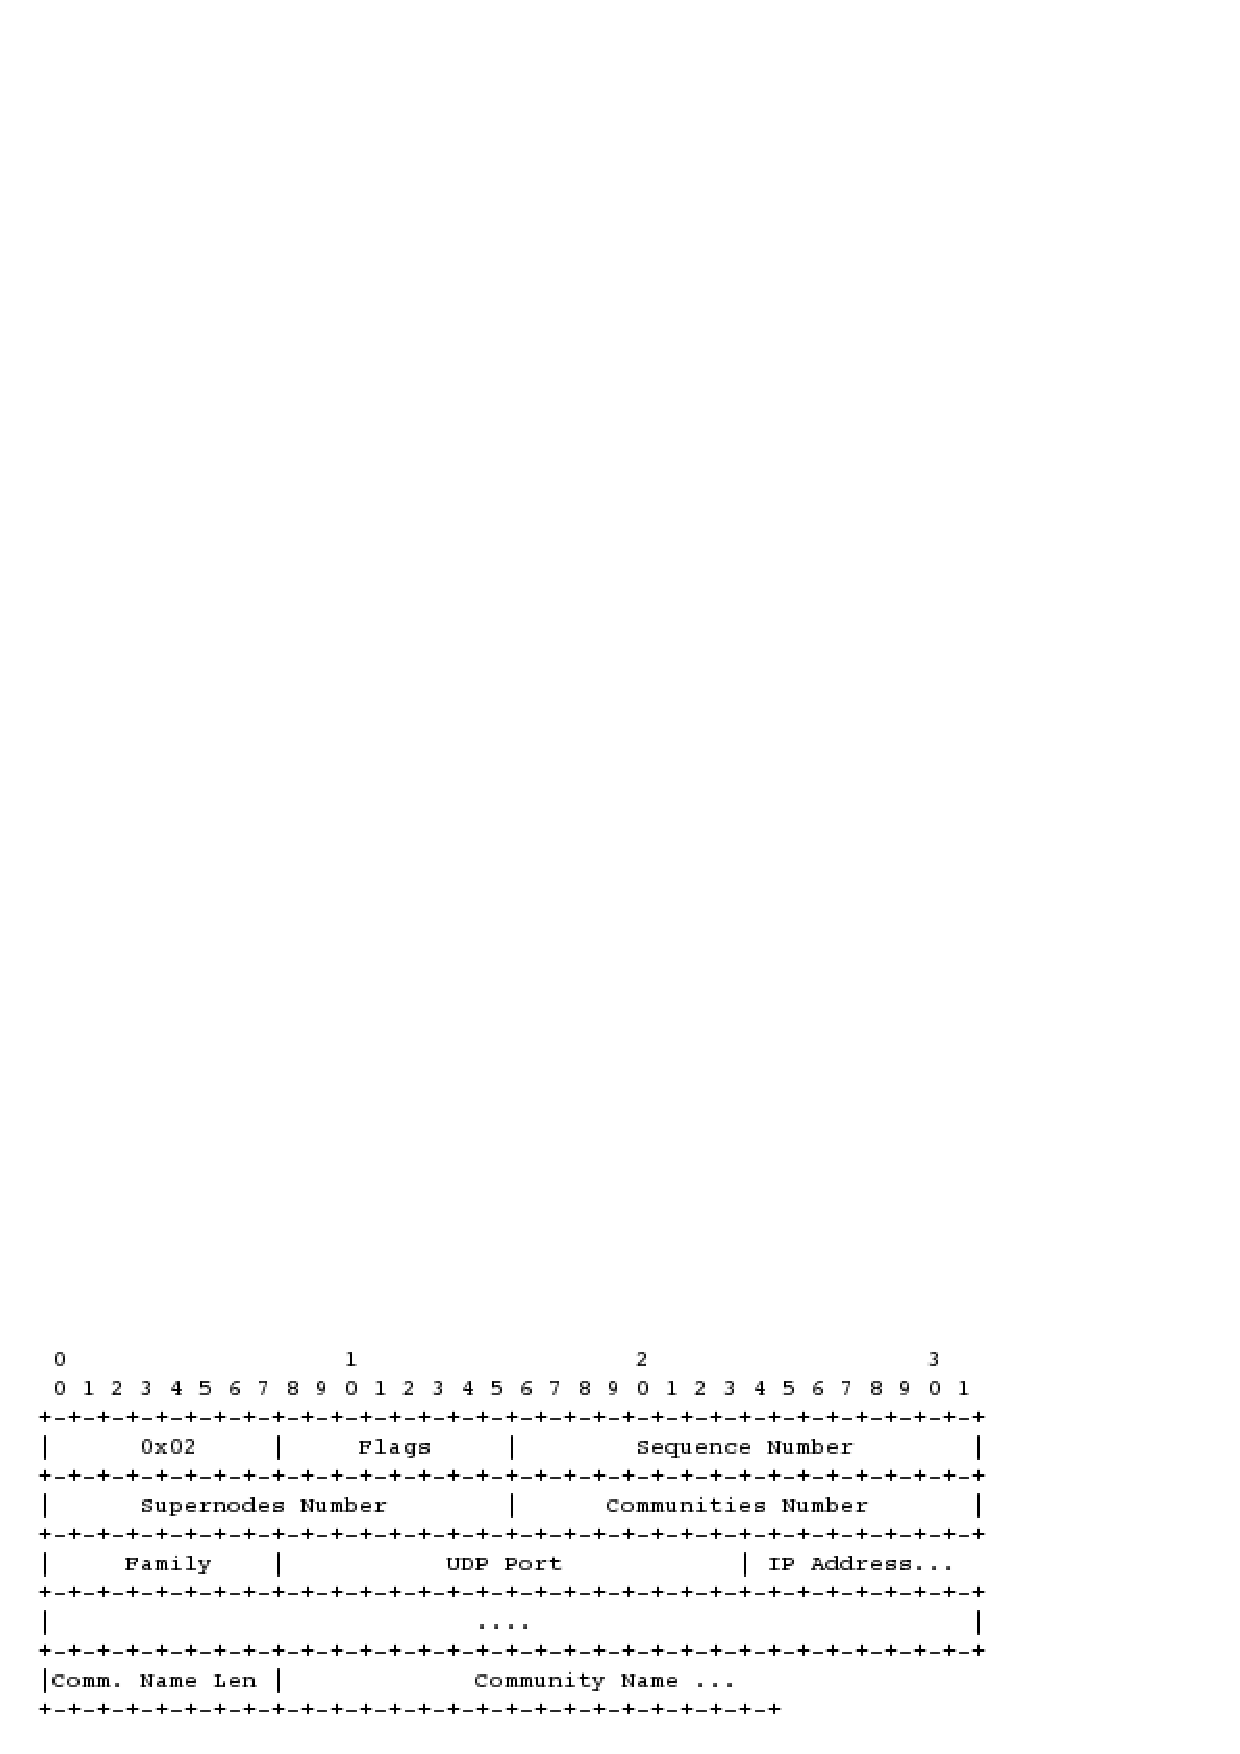
\includegraphics[scale=0.7]{img/snm-rsp.pdf}
\caption{SNM Response Message \label{img:snm-rsp}}
\end{center}
\end{figure}

If \emph{S} flag is set the response will contain SNM addresses of all known supernodes. If \emph{A} flag is set then the response will contain advertise addresses (N2N addresses) of supernodes coordinating a provided community. If \emph{N} flag is set, the supernodes addresses in the response are associated with an included community name. If \emph{C} flag is set, then the community names included in response are all those coordinated by responding supernode. If the response is sent to an edge-node, then when \emph{C} flag is set, only the community number is provided, considering that an edge will have no interest in other coordinated communities.

\subsection{SNM Advertise Message}
\label{sub-sec:snm-advertise}
The advertise message contains the advertise address of sending supernode and the names of communities coordinated by it. If the message is sent to another supernode, it may have the \emph{A} flag set, stating that sending supernode is also requesting for its counter-party advertise address. This may only happen during the community discovery stage of a starting supernode. A receiving supernode will advertise the sender in the registration acknowledgments sent to edges.

\begin{figure}[hbtp]
\begin{center}
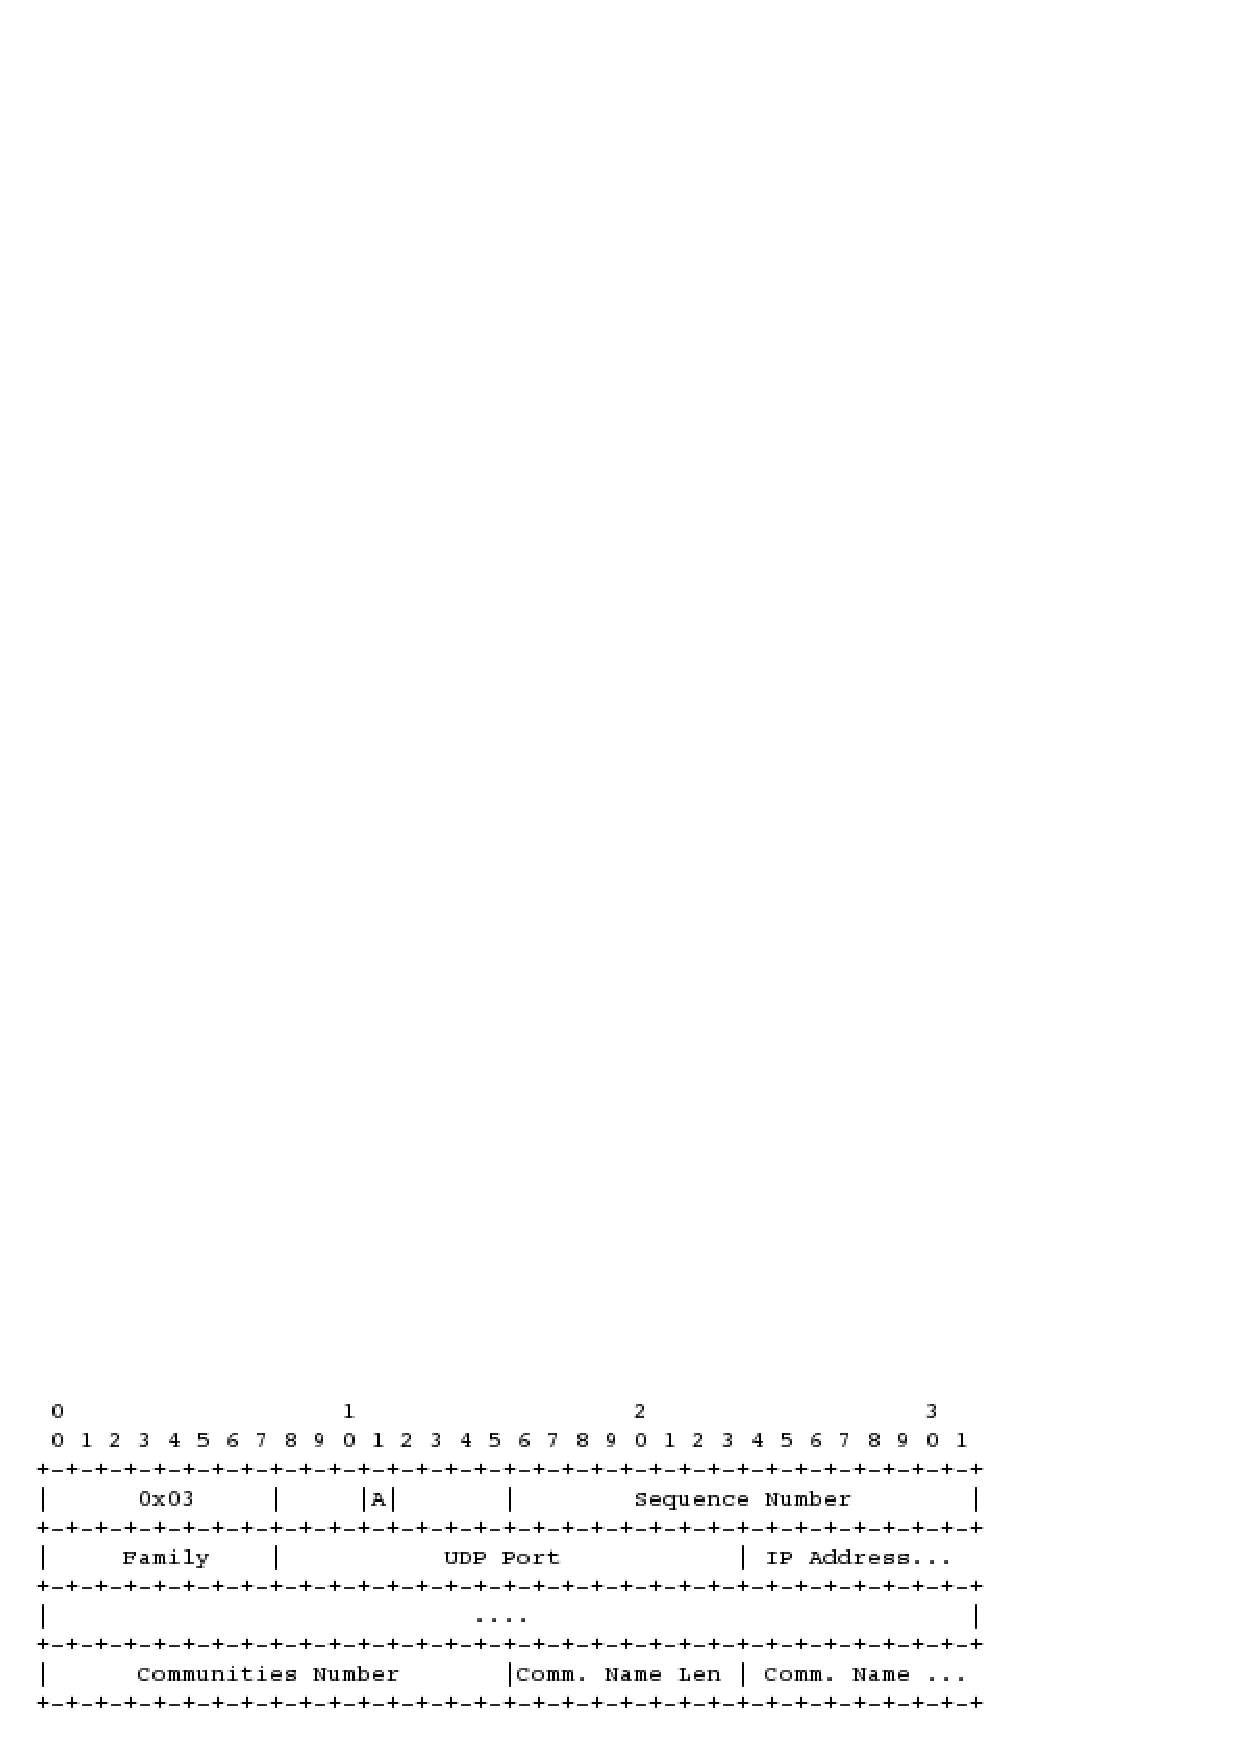
\includegraphics[scale=0.7]{img/snm-adv.pdf}
\caption{SNM Advertise Message \label{img:snm-adv}}
\end{center}
\end{figure}

\section{Supernodes Communication}
\label{sec:supernodes-communication}
% vim: set tw=78 sts=2 sw=2 ts=8 aw et ai:
Each supernode keeps a persistent list of all registered supernodes in a file, each entry having the form \emph{IP Address:Port}. On startup, a supernode will load the SNM addresses from file and will sent SNM requests to all of them. On first supernode startup it is mandatory to set the -i command line parameter value to a running supernode address (e.g. \emph{./supernode -i a.b.c.d:12000}). After all information about the other running supernodes is collected, the starting supernode will decide to send advertise messages to all those supernodes that are coordinating the communities it is interested in.

Coordinated communities are also kept in a file, along with the advertise addresses of the coordinating counter-parties. This information is also loaded on startup. The supernode will  run through the community discovery stage for finding those communities that have not acquired the needed level of redundancy. The requests will have the C flag set, demanding for communities coordinated by the queried supernode. After all the information is gathered, the new supernode will pick the communities which it will be coordinating, depending on the following parameters: 
\begin{itemize}
\item \emph{MIN_SN_per_COMM} – the minimum required number of supernodes coordinating a given community, needed for redundancy purpose 
\item \emph{MAX_SN_per_COMM} – the maximum number of supernodes serving a given community, needed for avoiding a given community being coordinated by all running supernodes 
\item \emph{MAX_COMM_per_SN} – the soft limit of communities being coordinated by a given supernode
\end{itemize}

\begin{figure}[hbtp]
\begin{center}
\includegraphics[scale=0.35]{img/supernode-bootstrap.pdf}
\caption{Communities discovery \label{img:supernode-bootstrap}}
\end{center}
\end{figure}

After deciding which communities it will voluntarily coordinate as well, advertise messages will be send to the coordinating counter-parties. The receivers will send back advertise messages with their N2N addresses. When receiving register messages from an edge-node, a supernode will fill in the acknowledgement message the advertising addresses of its counter-parties, to which the edge-node will send register messages also. This way, the lists of peers in the same community is also distributed to every coordinating supernode. An example of communities discovery stage is illustrated in \labelindexref{Fig.}{img:supernode-bootstrap}.

\section{Edge - Supernode Communication}
\label{sec:edge-supernode-communication}
% vim: set tw=78 sts=2 sw=2 ts=8 aw et ai:

The communication between edges and supernodes on the discovery stage was designed considering two options. First option was to integrate the SNM messages semantics in the existing N2N protocol. This solution would have involved that a supernode would have to handle SNM requests and responses under the N2N protocol as well. An edge-node would only connect to advertise addresses of supernodes, meaning that a coordinator assisting the edge bootstrap must keep track of all other supernodes advertise addresses as well.

The second option, that was chosen for the current implementation, implied using the SNM protocol for edge-supernode communication as well. The difference from the first option is that an edge must find the advertise addresses of supernodes coordinating its community. It has the advantage that it doesn't alter the existing N2N protocol and it keeps simplicity in the implementation. Sending back-up supernodes addresses to an edge was implemented by filling the supernode registration acknowledgments.

An edge-node starting for the first time, will begin in a discovery state, meaning that its main target will be to find the supernodes that will coordinate its community. There are 2 possible situations:
\begin{itemize}
\item the edge-node is initiating a new community and it will have to choose the supernodes that will coordinate it
\item the community already exists and the edge-node will discover the supernodes that are coordinating it
\end{itemize}
If the edge-node is initiating a new community, it will request the SNM address and communities number of every running supernode. After all information is collected, it will choose the supernodes that will be coordinating the new community. A supernode will be ranked based on  its communities number and its response time. Next, edge will start an advertise requesting stage receiving the advertise addresses of supernodes it has chosen. After all addresses are received, it will become ready from communication with community peers.

If the community already exists and the edge-node is starting for the first time, it will start discovering its community supernodes. The supernode discovery process will begin with sending requests to supernodes for that the SNM addresses were provided as command line parameters  (e.g. \emph{./edge -l  a.b.c.d:5645}). If a receiving supernode is coordinating the community, it will advertise its N2N address along with those of its counter-parties supernodes and the edge will become ready for processing messages from its peers. Otherwise, the supernode will send its communities number and the SNM addresses of all known supernodes.

After getting the complete list of coordinators' advertise addresses, the edge-node will be ready to process any incoming messages from its peers. Registration messages will be send to each supernode of the community in a round-robin fashion, that will help supernodes maintain the complete lists of community peers. A supernode registration acknowledgement will contain the advertising addresses of other coordinating supernodes as well. If a supernode will voluntarily decide to coordinate the community, its address will be advertised in the register acknowledgments. The list of community supernodes is saved in a file and loaded every subsequent next start-up.

The rank of a supernode is computed based on the response time and the load level that is represented by  number of coordinated communities. The formula used in ranking is:
\[
Rank = \frac{ResponseTime \cdot 100}{n},
\]
where \emph{n = MAX_COMM_per_SN – CommNum} if \emph{CommNum $<$ MAX_COMM_per_SN} or \emph{n = 1} otherwise.

The formula was chosen in order to offer a greater chance to supernodes having a lower number of communities. First \emph{MIN_SN_per_COMM} supernodes are chosen in from ascending ordered set of rankings. All supernodes advertise addresses will be kept in a file, each entry having the form \emph{IP Address:Port}.

All SNM messages added apply for edge-supernode communication. A SNM request initiated by an edge will have the \emph{E} (edge) flag set and will contain its community name. During supernode discovery stage, the edge-node will start sending requests for SNM addresses until the community supernodes set will be established. If the community is new, the edge will send requests for advertise to all the supernodes it decided to use.

A SNM response payload received by an edge-node may contain either SNM addresses or advertise addresses. The difference is given by the \emph{A} (advertise) flag, in which case the edge will use the addresses to register to supernodes. Upon receiving  such a response, the edge-node will stop quering for other supernodes SNM addresses and it will become ready for communicating with peers.

A SNM advertise message can only be received by an edge-node during discovery stage and only if it had previously requested it from a certain supernode.

\section{Experimental Setup}
\label{sec:setup}
% vim: set tw=78 sts=2 sw=2 ts=8 aw et ai:

In order to define recursion, one must first define recursion.


\section{Conclusion and Further Work}
\label{sec:conclusion}
% vim: set tw=78 sts=2 sw=2 ts=8 aw et ai:

The flexibility of multiple supernodes feature can be enhanced by adding other parameters to be included in the load balancing evaluation. When initiating a community, an edge may expand its set of potential supernodes if response times are under a configurable limit and choose them in a random way. Improving edge-nodes discovery and communication by using \emph{DHT}s may cancel out the need for supernodes, which would add full decentralization.
%\cite{large-scale-p2p-sim}.


\bibliography{multiple-supernodes}
\bibliographystyle{ieeetr}

\end{document}
